\documentclass[8pt]{beamer}
\usetheme{Madrid}
\usepackage[utf8]{inputenc}
\usepackage[spanish, es-tabla]{babel}
\usepackage{amsmath,amsfonts,amssymb,amsthm}
\usepackage{mathrsfs}
\usepackage{color}
\usepackage{xcolor, colortbl}
\usepackage{array, multirow, multicol}
\usepackage{graphicx}
\usepackage{epstopdf}
\usepackage{comment}
\usepackage{csquotes}
\usepackage{makecell}
\usepackage{booktabs}


% Bibliografía
\usepackage[backend=biber,style=authoryear]{biblatex}
\addbibresource{referencias_presentacion.bib}

% Separador de secciones automático
\AtBeginSection[]
{
\begin{frame}
\begin{Large}
\tableofcontents[sectionstyle=shaded,currentsection=show]
\end{Large}
\end{frame}
}

% Información de la presentación
\title[Entropía Relativa versus SLV]{Entropía Relativa versus Volatilidad Local Estocástica:\newline[0.2cm]
{\large Comparación de las dos estrategias dinámicas de cobertura}}
\author[Miriam Gutiérrez Serrano]{{\bf Autora:} Miriam Gutiérrez Serrano\newline
{\bf Tutor académico:} Carlos Vázquez Cendón (UDC)\newline
{\bf Tutor empresa:} Daniel Arrieta Rodríguez y Cristina Arribas Francisco\newline
\vspace{0.5cm} {\bf PFM Máster en Matemática Industrial}}

\date{Julio 2026}

%%%%%% INICIO PRESENTACIÓN %%%%%%%%%%%%
\begin{document}

%%%%%%%%%%%%%%%%%%%%%%%%%%%%%%%%%%%%%
%           PORTADA
%%%%%%%%%%%%%%%%%%%%%%%%%%%%%%%%%%%%%
\begin{frame}[plain]
\vspace*{-0.3cm}
\begin{center}
\begin{minipage}{3cm}
    
\includegraphics[width=2.8cm]{../memoria/logo_m2i}
\end{minipage}
\end{center}

\vspace{-0.1cm}
\begin{center}
\begin{minipage}{1.3cm}
    
\includegraphics[width=1.1cm]{../memoria/logo_ux}
\end{minipage}\hspace{0.1cm}
\begin{minipage}{2.2cm}
    
\includegraphics[width=2.2cm]{../memoria/logo_udc}
\end{minipage}\hspace{0.1cm}
\begin{minipage}{2cm}
    
\includegraphics[width=2cm]{../memoria/logo_uvigo}
\end{minipage}\hspace{0.1cm}
\begin{minipage}{2.4cm}
    
\includegraphics[width=2.4cm]{../memoria/logo_UC3M}
\end{minipage}\hspace{0.1cm}
\begin{minipage}{1.3cm}
    
\includegraphics[width=1.3cm]{../memoria/logo_UPM}
\end{minipage}
\end{center}

\vspace{0.2cm}
\begin{center}
{\small\bf PFM Máster en Matemática Industrial}\\[0.3cm]
{\large\bf Entropía Relativa versus Volatilidad Local Estocástica:}\\[0.1cm]
{\normalsize\bf Comparación de las dos estrategias dinámicas de cobertura}\\[0.4cm]
{\small Miriam Gutiérrez Serrano}\\[0.15cm]
{\scriptsize Tutor académico: Carlos Vázquez Cendón (UDC)\\
Tutor empresa: Daniel Arrieta Rodríguez y Cristina Arribas Francisco}\\[0.15cm]
{\scriptsize 
\includegraphics[width=3cm]{../memoria/Banco_Santander_Logotipo}}
\end{center}
\end{frame}

%%%%%%%%% INTRODUCCIÓN %%%%%%%%%%%
\begin{Large}
\begin{frame}{\bf {\LARGE {Introducción}}}
\begin{itemize}
    \item Valoración de productos derivados financieros.
    \pause
    \item {\bf Modelo de Black--Scholes} (1973)
    \pause
    \item {\bf Black Monday} (1987): desplome bursátil 
    \pause
    \item Necesidad de modelos más flexibles:
    \vspace{0.2cm}
    \begin{itemize}
        \item {\large \bf Volatilidad Local Estocástica (SLV)}
        \item {\large \bf Entropía Relativa Mínima (MRE)}
    \end{itemize}
\end{itemize}
\end{frame}
\end{Large}

\begin{frame}{Índice}
    \begin{Large}
\tableofcontents
\end{Large}
\end{frame}


%%%%%%%%%%%%%%%%%%%%%%%%%%%%%%%%%%%%%%%%%%%
% SECCIÓN 1: CONCEPTOS PRELIMINARES Y BLACK--SCHOLES
%%%%%%%%%%%%%%%%%%%%%%%%%%%%%%%%%%%%%%%%%%%
\section{Conceptos preliminares y Black--Scholes}

% Slide: Martingala y Teoremas Fundamentales
\begin{frame}{Martingala y valoración neutral al riesgo}
    Consideramos un espacio de probabilidad filtrado
    \[
    (\Omega , \mathcal{F},\{\mathcal{F}_t\}_{t\geq 0}, \mathbb{P})
    \]
    \pause
  \begin{block}{Definición (Martingala)}
    Un proceso estocástico $\{X(t)\}_{t \geq 0}$ es martingala respecto de la filtración $\{\mathcal F_t\}_{t\geq 0}$ y de la medida $\mathbb P$ si es adaptado, integrable y verifica
    \[
        \mathbb{E}^\mathbb{P}[X(T) | \mathcal{F}_t] = X(t), \quad t \leq T. 
    \]
  \end{block}
  \pause

  \begin{block}{Primer Teorema Fundamental de Valoración Financiera}
    Un mercado financiero está libre de arbitraje si y solo si existe una medida de probabilidad $\mathbb Q$, equivalente a $\mathbb{P}$, bajo la cual los precios descontados son martingalas:
    \[
        \frac{S^{(m)}(t)}{N(t)} = \mathbb{E}^\mathbb{Q}\left[ \frac{S^{(m)}(T)}{N(T)} \mid \mathcal{F}_t \right], \quad m = 1, \dots, M, \; t \leq T
    \]
  \end{block}
  
\end{frame}

%Slide: Mercado completo, incompleto y cambio de medida

\begin{frame}{Completitud y cambio de medida}

\begin{block}{Segundo Teorema Fundamental de Valoración Financiera}
Supongamos que el mercado está libre de arbitraje. Entonces, el mercado es completo si y solo si existe una única medida martingala equivalente.
\end{block}
\pause
\begin{itemize}
    \item Mercado completo:
    \begin{itemize}
        \item la medida de valoración es única;
        \item el precio de un derivado replicable queda determinado por ausencia de arbitraje.
    \end{itemize}

    \item Mercado incompleto:
    \begin{itemize}
        \item pueden existir varias medidas martingala equivalentes;
        \item puede haber distintos precios compatibles con ausencia de arbitraje.
    \end{itemize}
\end{itemize}
\pause
\begin{block}{Idea de cambio de medida}
Permite pasar de una medida real $\mathbb P$ a una medida de valoración $\mathbb Q$.
En procesos continuos, este cambio modifica el término de deriva del proceso.
\end{block}
\end{frame}

% Slide: Modelo de Black--Scholes
\begin{frame}{Modelo de Black--Scholes}

\begin{itemize}
    \item Bajo la medida real $\mathbb P$, el subyacente sigue
    \[
        dS(t)=\mu S(t)\,dt+\sigma S(t)\,dW^{\mathbb P}(t),
    \]
    donde $\mu$ es la rentabilidad esperada y $\sigma>0$ es constante.
    \pause
    \item Para valorar derivados se trabaja bajo la medida neutral al riesgo $\mathbb Q$:
    \[
        dS(t)=rS(t)\,dt+\sigma S(t)\,dW^{\mathbb Q}(t).
    \]

    \item El cambio de medida sustituye la deriva real $\mu$ por el tipo libre de riesgo $r$.
\end{itemize}
\pause
\begin{block}{Fórmula de Black--Scholes para opciones Call y Put europeas}
\[
    C_{BS}=S_0\Phi(d_1)-Ke^{-rT}\Phi(d_2),
\]
\[
    P_{BS}=Ke^{-rT}\Phi(-d_2)-S_0\Phi(-d_1),
\]
donde
\[
    d_1=
    \frac{\log(S_0/K)+(r+\frac{1}{2}\sigma^2)T}{\sigma\sqrt{T}},
    \qquad
    d_2=d_1-\sigma\sqrt{T}.
\]
\end{block}

\end{frame}

% Slide: Volatilidad implícita y limitaciones
\begin{frame}{Volatilidad implícita y limitaciones}

\begin{block}{Definición (Volatilidad implícita)}
Dado un precio de mercado $C^{mkt}(K,T)$, la volatilidad implícita 
$\sigma_{imp}(K,T)$ es el valor que verifica
\[
    C_{BS}(S_0,K,T,r,\sigma_{imp}(K,T))=C^{mkt}(K,T).
\]
\end{block}
\pause
\begin{itemize}
    \item Si Black--Scholes describiera perfectamente el mercado:
    \[
        \sigma_{imp}(K,T) \text{ sería constante.}
    \]

    \item En la práctica:
    \[
        \sigma_{imp}(K,T) \text{ depende del strike y del vencimiento.}
    \]

    \item Para un vencimiento fijo aparece el \textbf{smile} o \textbf{skew} de volatilidad.

    \item Para varios vencimientos se obtiene la \textbf{superficie de volatilidad implícita}.

    \item Esto motiva el estudio de modelos más flexibles.
\end{itemize}

\end{frame}

%Slide: Opciones forward-start
\begin{frame}{Opciones forward-start}
    \begin{block}{Definición (opción forward-start)}
        Una opción \textit{forward-start} es un derivado cuyo periodo de referencia comienza en una fecha futura $T_1$ y vence en una fecha posterior $T_2$, con $0<T_1<T_2$. En particular, una call (put) con strike relativo $K$ tiene payoff
        \[
            \max\{S(T_2)-KS(T_1,0)\}\quad (\max\{KS(T_1)-S(T_2),0)\})
        \]
    \end{block}
    \pause
    \begin{itemize}
    

        \item Versión normalizada Call:
        \[
            \max\left\{\frac{S(T_2)}{S(T_1)}-K,0\right\}.
        \]

        \item Su precio bajo la medida neutral al riesgo es
        \[
            C_{FS}=e^{-rT_2}
            \mathbb{E}^{\mathbb Q}\left[
            \max\left\{\frac{S(T_2)}{S(T_1)}-K,0\right\}
            \right], \text{ y }
        \]
        \[
            P_{FS}=e^{-rT_2}
            \mathbb{E}^{\mathbb Q}\left[
            \max\left\{K-\frac{S(T_2)}{S(T_1)},0\right\}
            \right].
        \]

        \item Sensibles a la dinámica futura de la volatilidad.
    \end{itemize}

\end{frame}

%%%%%%%%%%%%%%%%%%%%%%%%%%%%%%%%%%%%%%%%%%%
% SECCIÓN 2: VOLATILIDAD LOCAL ESTOCÁSTICA
%%%%%%%%%%%%%%%%%%%%%%%%%%%%%%%%%%%%%%%%%%%
\section{Volatilidad Local Estocástica}

% Slide: Volatilidad local y Dupire
\begin{frame}{Volatilidad Local: Fórmula de Dupire}
    Reemplazar $\sigma$ constante por una función $\sigma_{LV}(S,t)$:
    \[
        dS(t) = rS(t)\,dt + \sigma_{LV}(S(t),t)S(t)\,dW(t)
    \]
    \pause
    
    \begin{block}{Fórmula de Dupire}
        La varianza local se obtiene a partir de la superficie de precios de opciones:
        \[
            \sigma_{LV}^2(K,T) = \frac{\dfrac{\partial V_c}{\partial T} + rK\dfrac{\partial V_c}{\partial K}}{\dfrac{1}{2}K^2\dfrac{\partial^2 V_c}{\partial K^2}}
        \]
    \end{block}
    \pause
    
    \vspace{0.3cm}
    \textbf{Ventaja:} Ajuste exacto a opciones vanilla de mercado.\\[0.2cm]
    \textbf{Limitación:} Volatilidad determinista $\Longrightarrow$ no modela la evolución futura estocástica de la volatilidad.
\end{frame}


% Slide: Modelo de Heston
\begin{frame}{Volatilidad Estocástica: Modelo de Heston}
    Bajo la medida neutral al riesgo $\mathbb{Q}$:
    \begin{block}{Modelo de Heston}
    \[
    \begin{cases}
    dS(t) = rS(t)\,dt+\sqrt{v(t)}S(t)\,dW^{S}(t), \\[0.15cm]
    dv(t) = \kappa(\theta-v(t))\,dt+\gamma\sqrt{v(t)}\,dW^{v}(t),\\[0.15cm]
    dW^{S}(t)\,dW^{v}(t)=\rho_{S,v}\,dt.
    \end{cases}
    \]
    \end{block}
    \pause
    
    \vspace{0.2cm}
    \textbf{Parámetros:}
    \begin{itemize}
        \item $\kappa$: velocidad de reversión a la media
        \item $\theta$: nivel medio de largo plazo de la varianza
        \item $\gamma$: volatilidad de la volatilidad (vol-of-vol)
        \item $\rho_{S,v}$: correlación subyacente--varianza
        \item $v_0$: varianza inicial
    \end{itemize}
    \pause
    
    \vspace{0.2cm}
    \textbf{Condición de Feller} (positividad de $v(t)$): $2\kappa\theta \geq \gamma^2$
    
    \vspace{0.2cm}
    \textbf{Limitación:} Solo 5 parámetros $\Longrightarrow$ ajuste limitado a la superficie completa.
\end{frame}

% Slide: Condición de Feller
\begin{frame}{Condición de Feller en el proceso CIR}
    \begin{center}
        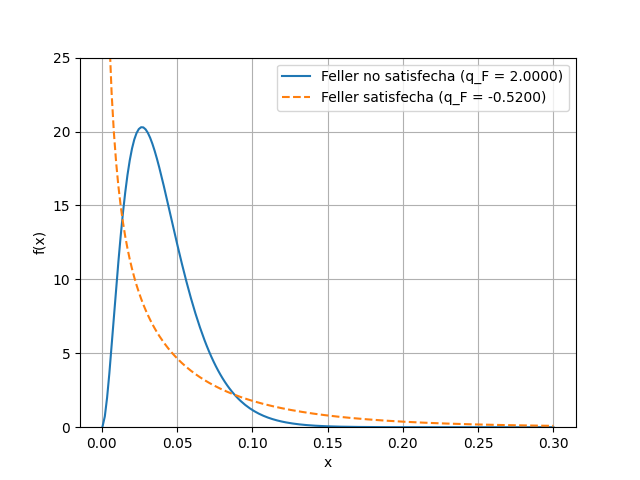
\includegraphics[width=0.58\textwidth]{../results/cir_feller_density.png}
    \end{center}
    \vspace{-0.2cm}
    \begin{center}
    {\small Densidad de transición del proceso CIR bajo dos parametrizaciones respecto a la condición de Feller.}
    \end{center}
    \pause
    
    \vspace{0.1cm}
    \begin{itemize}
        \item La condición de Feller controla el comportamiento de la varianza cerca de cero.
        \item Es relevante para la estabilidad numérica de la componente Heston del modelo SLV.
    \end{itemize}
\end{frame}


% Slide: Modelo Heston--SLV
\begin{frame}{Modelo Heston--SLV}
    Combina volatilidad local + estocástica:
    \begin{block}{Modelo Heston--SLV}
    \[
    \begin{cases}
    \dfrac{dS(t)}{S(t)} = r\,dt+\eta(S(t),t)\sqrt{v(t)}\,dW^S(t), \\[0.25cm]
    dv(t) = \kappa(\theta-v(t))\,dt+\gamma\sqrt{v(t)}\,dW^v(t), \\[0.25cm]
    dW^S(t)\,dW^v(t)=\rho_{S,v}\,dt.
    \end{cases}
    \]
    \end{block}
    \pause
    
    \begin{block}{Función de apalancamiento (leverage function)}
        La condición de proyección markoviana impone:
        \[
            \sigma_{LV}^2(K,t) = \eta^2(K,t)\cdot\mathbb{E}^\mathbb{Q}\left[v(t) \mid S(t)=K\right]
        \]
        Por tanto:
        \[
            \boxed{\eta(K,t) = \frac{\sigma_{LV}(K,t)}{\sqrt{\mathbb{E}^\mathbb{Q}\left[v(t) \mid S(t)=K\right]}}}
        \]
    \end{block}
    \pause
    
    $\Longrightarrow$ \textbf{Ajuste exacto a la superficie} (vía $\eta$) + \textbf{dinámica estocástica} (vía Heston).
\end{frame}


%%%%%%%%%%%%%%%%%%%%%%%%%%%%%%%%%%%%%%%%%%%
% SECCIÓN 3: ENTROPÍA RELATIVA Y WMC
%%%%%%%%%%%%%%%%%%%%%%%%%%%%%%%%%%%%%%%%%%%
\section{Entropía Relativa y Weighted Monte Carlo}

% Slide: Entropía relativa
\begin{frame}{Entropía relativa (Divergencia de Kullback--Leibler)}
    \begin{block}{Definición (Entropía relativa)}
        Sean $\mathbb{P}$ y $\mathbb{Q}$ dos medidas de probabilidad sobre $(\Omega,\mathcal{F})$. La entropía relativa de $\mathbb{Q}$ respecto de $\mathbb{P}$ es:
        \[
            D(\mathbb{Q}\|\mathbb{P}) = \sum_{\omega\in\Omega} q(\omega)\log\left(\frac{q(\omega)}{p(\omega)}\right)
        \]
    \end{block}
    \pause
    
    \textbf{Propiedades:} $D \geq 0$, $D = 0 \Leftrightarrow \mathbb{Q} = \mathbb{P}$, no simétrica.
    \pause
    
    \vspace{0.3cm}
    \begin{block}{Problema de Entropía Relativa Mínima (MRE)}
        \[
            \min_{\mathbb{Q}\in\mathcal{Q}} D(\mathbb{Q}\|\mathbb{P}) \quad \text{sujeto a} \quad \mathbb{E}^\mathbb{Q}[g_j(\omega)] = c_j, \quad j=1,\ldots,m
        \]
    \end{block}
    \pause
    
    \vspace{0.2cm}
    $\Longrightarrow$ Entre todas las medidas que reproducen las restricciones de mercado, se selecciona la \textbf{más cercana} a la medida previa $\mathbb{P}$.
\end{frame}

% Slide: Weighted Monte Carlo
\begin{frame}{Weighted Monte Carlo}
    \textbf{Idea:} Mantener fijas las $N$ trayectorias simuladas y modificar sus probabilidades.
    \pause
    
    \vspace{0.2cm}
    \begin{itemize}
        \item Monte Carlo estándar: $p_i = 1/N$ (pesos uniformes)
        \item WMC: buscar nuevos pesos $q = (q_1,\ldots,q_N)$
    \end{itemize}
    \pause
    
    \begin{block}{Restricciones de calibración}
        \[
            \sum_{i=1}^N q_i g_{ij} = C_j, \quad j=1,\ldots,m, \quad \sum_{i=1}^N q_i = 1, \quad q_i \geq 0
        \]
    \end{block}
    \pause
    
    \begin{block}{Pesos óptimos (forma de Boltzmann--Gibbs)}
        \[
            q_i = \frac{p_i\exp\left(\sum_{j=1}^m \lambda_j g_{ij}\right)}{Z(\lambda)}, \quad Z(\lambda) = \sum_{i=1}^N p_i\exp\left(\sum_{j=1}^m \lambda_j g_{ij}\right)
        \]
    \end{block}
    \pause
    
    Problema dual sin restricciones: $\displaystyle\min_{\lambda\in\mathbb{R}^m} W(\lambda) = \log Z(\lambda) - \sum_{j} \lambda_j C_j$
\end{frame}

% Slide: Ajuste exacto vs mínimos cuadrados ponderados
\begin{frame}{Ajuste exacto vs. Mínimos cuadrados ponderados}
    \begin{columns}[T]
    \begin{column}{0.48\textwidth}
    \textbf{Ajuste exacto:}
    \begin{itemize}
        \item Restricciones rígidas: $G^\top q = C$
        \item Máxima consistencia
        \item Puede ser inestable si hay muchas restricciones
    \end{itemize}
    \end{column}
    \begin{column}{0.48\textwidth}
    \textbf{Mínimos cuadrados ponderados:}
    \begin{itemize}
        \item Regularización:
        \[
            H(\lambda) = W(\lambda) + \frac{1}{2}\lambda^\top\Omega\lambda
        \]
        \item Tolerancia controlada
        \item Mayor estabilidad numérica
    \end{itemize}
    \end{column}
    \end{columns}
    \pause
    
    \vspace{0.4cm}
    \textbf{Resolución numérica:} Método de Newton amortiguado
    \[
        \lambda^{(k+1)} = \lambda^{(k)} - \alpha\, d^{(k)}, \quad J(\lambda^{(k)})d^{(k)} = \nabla W(\lambda^{(k)})
    \]
    \pause
    
    \vspace{0.2cm}
    \textbf{Salvaguardas numéricas:}
    \begin{itemize}
        \item Evaluación estable de $\log Z(\lambda)$ (log-sum-exp)
        \item Regularización diagonal, resolución por mínimos cuadrados si sistema mal condicionado
        \item Amortiguación adaptativa: $\alpha_0 = 0.01$, $\alpha_{\max} = 1$
    \end{itemize}
\end{frame}


%%%%%%%%%%%%%%%%%%%%%%%%%%%%%%%%%%%%%%%%%%%
% SECCIÓN 4: IMPLEMENTACIÓN NUMÉRICA Y RESULTADOS
%%%%%%%%%%%%%%%%%%%%%%%%%%%%%%%%%%%%%%%%%%%
\section{Implementación numérica y resultados}

% Slide: Datos de entrada
\begin{frame}{Datos de entrada}
    \begin{itemize}
        \item $S_0 = 100$, $r = 0$, $q = 0$
        \item Superficie de volatilidades implícitas de Oosterlee et al. (2021)
    \end{itemize}
    
    \vspace{0.2cm}
    \begin{table}
    \centering
    \scriptsize
    \begin{tabular}{c|cccccccc}
    \hline
    \textbf{Strike/T} & \textbf{1w} & \textbf{1m} & \textbf{6m} & \textbf{1y} & \textbf{2y} & \textbf{5y} & \textbf{8y} & \textbf{10y} \\
    \hline
    40  & 22.62 & 22.37 & 20.71 & 18.54 & 18.04 & 16.40 & 14.49 & 13.14 \\
    60  & 15.49 & 15.35 & 14.42 & 13.20 & 12.92 & 11.99 & 10.92 & 10.18 \\
    80  & 9.93  & 9.88  & 9.56  & 9.15  & 9.07  & 8.79  & 8.46  & 8.25  \\
    100 & 5.00  & 5.07  & 5.52  & 6.04  & 6.20  & 6.64  & 7.02  & 7.22  \\
    120 & 4.54  & 4.60  & 4.96  & 5.43  & 5.65  & 6.28  & 6.78  & 7.04  \\
    140 & 6.28  & 6.30  & 6.41  & 6.46  & 6.61  & 6.98  & 7.23  & 7.33  \\
    160 & 7.75  & 7.75  & 7.71  & 7.52  & 7.62  & 7.81  & 7.82  & 7.75  \\
    \hline
    \end{tabular}
    \caption{Superficie de volatilidades implícitas (\%).}
    \end{table}
    
    \pause
    \vspace{0.1cm}
    Precios de referencia: $C_{ij}^{mkt} = C^{BS}(S_0, K_j, T_i, r, \sigma_{imp}(T_i,K_j))$
\end{frame}

% Slide: Calibración Heston-SLV
\begin{frame}{Calibración del modelo Heston--SLV}
    \textbf{Paso 1: Calibración de la componente Heston} (método COS)
    \[
        \min_{\kappa,\theta,\gamma,\rho_{S,v},v_0} \left(\sum_{i,j}\left(C_{ij}^{Heston} - C_{ij}^{mkt}\right)^2\right)^{1/2}
    \]
    \pause
    
    \begin{table}
    \centering
    \begin{tabular}{ccccc}
    \hline
    $\kappa$ & $\theta$ & $\gamma$ & $\rho_{S,v}$ & $v_0$ \\
    \hline
    $2.12$ & $0.06$ & $0.16$ & $-0.71$ & $0.001$ \\
    \hline
    \end{tabular}
    \caption{Parámetros calibrados de la componente Heston.}
    \end{table}
    \pause
    
    \textbf{Paso 2: Función de apalancamiento $\eta(K,t)$}
    \begin{itemize}
        \item Superficie de volatilidad local $\sigma_{LV}$ vía Dupire (interpolación cúbica Hermite, $\Delta K = 2.5$)
        \item $\mathbb{E}[v(t)|S(t)=K]$ estimada por \textit{binning} durante simulación MC
    \end{itemize}
    \pause
    
    \textbf{Paso 3: Simulación Monte Carlo}
    \begin{itemize}
        \item Esquemas Euler y AES $\Longrightarrow$ resultados prácticamente coincidentes
        \item Reescalado: $\mathbb{E}[S(t)] = S_0 e^{rt}$
    \end{itemize}
\end{frame}

% Slide: Comparación Euler vs AES
\begin{frame}{Comparación Euler vs. AES}
    \begin{center}
        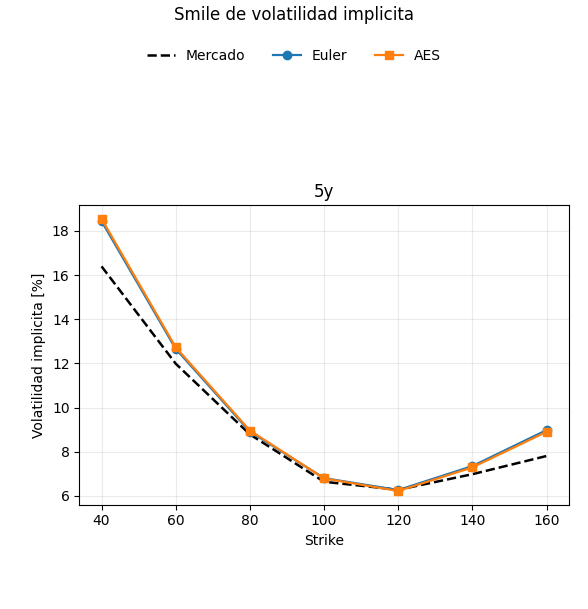
\includegraphics[width=0.47\textwidth]{../results/AES_vs_Euler_5y.png}
    \end{center}
    \vspace{-0.2cm}
    \begin{center}
    {\small Smile de volatilidad implícita para $T=5$ años: Euler vs. AES vs. mercado.}
    \end{center}
    
    \vspace{0.05cm}
    \begin{itemize}
        \item Ambos esquemas reproducen adecuadamente el smile de mercado
        \item Diferencias reducidas $\Longrightarrow$ se utiliza Euler en los resultados finales
    \end{itemize}
\end{frame}

% Slide: Implementación MRE
\begin{frame}{Implementación del método MRE/WMC}
    \textbf{Configuración:}
    \begin{itemize}
        \item $N = 20\,000$ trayectorias lognormales, semilla fija $12345$, variables antitéticas
        \item Volatilidad prior: estructura temporal ATM
        \item Precios benchmark: los obtenidos con Heston--SLV
    \end{itemize}
    \pause
    
    \textbf{Restricciones de calibración:}
    \begin{enumerate}
        \item Precios de opciones call ($K \in \{40,60,80,100,120,140\}$, 8 vencimientos)
        \item Restricciones forward: $\sum q_i S_i(T_j) = S_0$
        \item Restricciones sintéticas de martingala entre vencimientos
    \end{enumerate}
    \pause
    
    \textbf{Resolución:} Newton amortiguado, tolerancia gradiente $10^{-8}$, tolerancia precios $5\cdot 10^{-4}$
    \pause
    
    \begin{table}
    \centering
    \begin{tabular}{c|ccc}
    \hline
     & Mínimo & Media & Máximo \\
    \hline
    $q_i$ & $2.62\cdot 10^{-25}$ & $5.00\cdot 10^{-5}$ & $1.79\cdot 10^{-3}$ \\
    \hline
    \end{tabular}
    \caption{Pesos posteriores MRE.}
    \end{table}
\end{frame}

% Slide: Comparación opciones vanilla
\begin{frame}{Comparación: opciones europeas vanilla}
    Strikes \textbf{no utilizados} como benchmark: $K \in \{70, 90, 110\}$
    
    \begin{table}
    \centering
    \small
    \begin{tabular}{|c|c|c|}
    \hline
     \textbf{Vencimiento} & \textbf{MAE} & \textbf{Dif. máxima} \\
    \hline
     0.02  & 0.0000 & 0.0000 \\
     0.08  & 0.0000 & 0.0000 \\
     0.50  & 0.0533 & 0.0900 \\
     1.00  & 0.1567 & 0.2900 \\
     2.00  & 0.1900 & 0.2800 \\
     5.00  & 0.2933 & 0.4200 \\
     8.00  & 0.3500 & 0.6600 \\
     10.00 & 0.3300 & 0.6700 \\
    \hline
    \end{tabular}
    \caption{MAE (WMC vs. Heston--SLV) por vencimiento.}
    \end{table}
    \pause
    
    \vspace{0.1cm}
    \begin{itemize}
        \item \textbf{MAE global $\approx 0.17$}: diferencias moderadas
        \item Vencimientos cortos: coincidencia prácticamente exacta
        \item Diferencias crecen con el vencimiento, pero se mantienen contenidas
    \end{itemize}
\end{frame}

% Slide: Comparación forward-start
\begin{frame}{Comparación: opciones forward-start}
    $K \in \{70, 90, 110\}$, 10 pares $(T_1,T_2)$
    
    \begin{table}
    \centering
    \small
    \begin{tabular}{|c|c|c|c|}
    \hline
    $T_1$ & $T_2$ & \textbf{MAE} & \textbf{Dif. máxima} \\
    \hline
    0.50 & 1.00  & 0.0767 & 0.1400 \\
    0.50 & 2.00  & 0.1967 & 0.3700 \\
    0.50 & 5.00  & 0.3400 & 0.5500 \\
    0.50 & 10.00 & 0.3767 & 0.7000 \\
    1.00 & 2.00  & 0.1700 & 0.3800 \\
    1.00 & 5.00  & 0.3933 & 0.6600 \\
    1.00 & 10.00 & 0.3833 & 0.7300 \\
    2.00 & 5.00  & 0.3400 & 0.5600 \\
    2.00 & 10.00 & 0.3600 & 0.5900 \\
    5.00 & 10.00 & 0.3067 & 0.3900 \\
    \hline
    \end{tabular}
    \caption{MAE (WMC vs. Heston--SLV) por par $(T_1,T_2)$.}
    \end{table}
    \pause
    
    \begin{itemize}
        \item \textbf{MAE global $\approx 0.29$}: mayor que en opciones vanilla
        \item Diferencias crecen al aumentar $T_2$ para $T_1$ fijo
    \end{itemize}
\end{frame}

% Slide: Smile forward-start
\begin{frame}{Smile forward-start y formulación regularizada}
    \begin{center}
        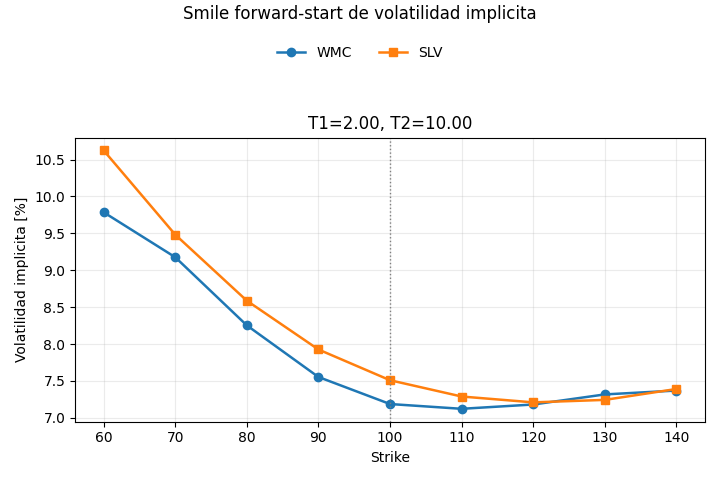
\includegraphics[width=0.6\textwidth]{../results/wmc-slv_forward_start_WLS.png}
    \end{center}
    \vspace{-0.2cm}
    \begin{center}
    {\small Smile forward-start ($T_1=2$, $T_2=10$): WMC (mínimos cuadrados ponderados) vs. Heston--SLV.}
    \end{center}
    \pause
    
    \vspace{0.2cm}
    \begin{itemize}
        \item Ajuste exacto: problemas de estabilidad para el smile forward-start
        \item Mínimos cuadrados ponderados ($\omega = 10^{-7}$): estructura del smile más estable
        \item \textbf{Proximidad en precios $\neq$ buena reproducción de la estructura de volatilidad implícita}
    \end{itemize}
\end{frame}


%%%%%%%%%%%%%%%%%%%%%%%%%%%%%%%%%%%%%%%%%%%
% SECCIÓN 5: CONCLUSIONES
%%%%%%%%%%%%%%%%%%%%%%%%%%%%%%%%%%%%%%%%%%%
\section{Conclusiones y líneas futuras}

\begin{frame}{Conclusiones}
    \begin{enumerate}
        \item Ambas metodologías incorporan la información de la superficie de volatilidad, pero desde \textbf{perspectivas diferentes}:
        \begin{itemize}
            \item \textbf{Heston--SLV}: modifica la dinámica del subyacente (componente local + estocástica)
            \item \textbf{MRE/WMC}: mantiene trayectorias fijas y redistribuye probabilidades
        \end{itemize}
        \pause
        
        \item Para \textbf{opciones vanilla}, MRE reproduce razonablemente los precios SLV (MAE $\approx 0.17$), incluso en strikes no utilizados como benchmark
        \pause
        
        \item Para \textbf{opciones forward-start}:
        \begin{itemize}
            \item Los precios son relativamente próximos (MAE $\approx 0.29$)
            \item Pero la estructura del smile forward muestra diferencias significativas
            \item El ajuste exacto es inestable; la formulación regularizada (WLS) es más robusta
        \end{itemize}
        \pause
        
        \item \textbf{Conclusión principal:} la proximidad en precios no garantiza una buena reproducción de la estructura de volatilidad implícita. Las opciones forward-start revelan diferencias que no se aprecian con opciones vanilla
    \end{enumerate}
\end{frame}

\begin{frame}{Líneas futuras de investigación}
    \begin{enumerate}
        \item \textbf{Datos reales de mercado}: aplicar ambas metodologías a superficies de volatilidad observadas en distintos activos y fechas
        \pause
        
        \item \textbf{Productos más complejos}: opciones asiáticas, opciones barrera, productos dependientes de la trayectoria
        \pause
        
        \item \textbf{Análisis de cobertura}: estudio de las sensibilidades (Griegas) y la estabilidad de las estrategias de cobertura
        \pause
        
        \item \textbf{Extensiones del método MRE}: comparación con Generalized Weighted Monte Carlo u otros métodos de calibración basados en optimización
    \end{enumerate}
\end{frame}


%%%%%%%%%%%%%%%%%%%%% REFERENCIAS %%%%%%%%%%%%%%%%%%%%%%%
\begin{frame}{\bf Referencias}
\begin{thebibliography}{50}
\scriptsize

  \bibitem{ref:oosterlee} Oosterlee, C.W., Grzelak, L.A., Leitao, Á.
  {\em Modelos matemáticos y métodos numéricos en finanzas cuantitativas}. Editorial Aula Magna, 2021.

  \bibitem{ref:avellaneda} Avellaneda, M. et al.
  {\em Weighted Monte Carlo: A New Technique for Calibrating Asset-Pricing Models}. IJTAF, 4(1), 2001.

  \bibitem{ref:elices} Elices, A. y Giménez, E.
  {\em Weighted Monte Carlo: Calibrating the Smile and Preserving Martingale Condition}. SSRN, 2011.

  \bibitem{ref:arrieta} Arrieta, D.
  {\em SLV vs Relative Entropy: Two Perfect Models Comparison}. Presentation, 2024.

  \bibitem{ref:dupire} Dupire, B.
  {\em Pricing with a smile}. Risk 7, 1994.

  \bibitem{ref:vazquez} Vázquez, C.
  {\em An Introduction to Black-Scholes Modeling}. MAT Serie A, 17, 2010.

\end{thebibliography}
\end{frame}



%%%%%%%%%%%%%%%%% FIN %%%%%%%%%%%%%%%%%%%%%%%
\begin{frame}[plain]
\vspace*{-0.3cm}
\begin{center}
\begin{minipage}{3cm}
    
\includegraphics[width=2.8cm]{../memoria/logo_m2i}
\end{minipage}
\end{center}

\vspace{-0.1cm}
\begin{center}
\begin{minipage}{1.3cm}
    
\includegraphics[width=1.1cm]{../memoria/logo_ux}
\end{minipage}\hspace{0.1cm}
\begin{minipage}{2.2cm}
    
\includegraphics[width=2.2cm]{../memoria/logo_udc}
\end{minipage}\hspace{0.1cm}
\begin{minipage}{2cm}
    
\includegraphics[width=2cm]{../memoria/logo_uvigo}
\end{minipage}\hspace{0.1cm}
\begin{minipage}{2.4cm}
    
\includegraphics[width=2.4cm]{../memoria/logo_UC3M}
\end{minipage}\hspace{0.1cm}
\begin{minipage}{1.3cm}
    
\includegraphics[width=1.3cm]{../memoria/logo_UPM}
\end{minipage}
\end{center}

\vspace{0.2cm}
\begin{center}
{\small\bf PFM Máster en Matemática Industrial}\\[0.3cm]
{\large\bf Entropía Relativa versus Volatilidad Local Estocástica:}\\[0.1cm]
{\normalsize\bf Comparación de las dos estrategias dinámicas de cobertura}\\[0.4cm]
{\small Miriam Gutiérrez Serrano}\\[0.15cm]
{\scriptsize Tutor académico: Carlos Vázquez Cendón (UDC)\\
Tutor empresa: Daniel Arrieta Rodríguez y Cristina Arribas Francisco}\\[0.15cm]
{\scriptsize 
\includegraphics[width=3cm]{../memoria/Banco_Santander_Logotipo}}
\end{center}
\end{frame}

\end{document}
